\graphicspath{{Figs/sensor/}}

\chapter{Sensor modeling}
 \label{sec:sensor}

%
% Document history, format:
%  \starthistory
%    date1 & text .... \\
%    date2 & text .... \\
%    ....
%  \stophistory
%
\starthistory
  050121 & Revised and extended by Mattias Ekstr\"om. \\
  000826 & Written for ARTS-1 by Patrick Eriksson.\\
\stophistory


%
% Symbol table, format:
%  \startsymbols
%    ... & \verb|...| & text ... \\
%    ... & \verb|...| & text ... \\
%    ....
%  \stopsymbols
%
%
\startsymbols
$w_\mathrm{a}$  & \artsstyle{antenna\_diagram} & The antenna pattern \\
$w_\mathrm{b}$ & & The backend channel response \\
$w_\mathrm{sb}$ & & The sideband filter function\\
%   & \artsstyle{antenna\_dim} & The dimensionality of the antenna pattern \\
\aFrq{ch}  & \artsstyle{f\_backend} & The frequency grid of the backend channels \\
%   & \artsstyle{f\_mixer} & Output frequency grid from the mixer \\
\aFrq{\mathrm{LO}}  & \artsstyle{lo} & Local oscillator frequency \\
% \AzmAng & \artsstyle{mblock\_za\_grid} & The zenith angle grid for each measurement block \\
% \ZntAng & \artsstyle{mblock\_aa\_grid} & The azimuthal angle grid for each measurement block \\
\MtrStl{P} & \artsstyle{sensor\_pol} & The sensor polarisation response \\
\SnsMtr & \artsstyle{sensor\_response} & The total sensor response matrix \\
%   & \artsstyle{sensor\_response\_f} & The sensor frequency grid \\
%   & \artsstyle{sensor\_response\_za} & The sensor zenith angle grid \\
%   & \artsstyle{sensor\_response\_aa} & The sensor azimuth angle grid \\
%   & \artsstyle{sensor\_rot} & The rotation of the sensor between measurement blocks \\
 \label{symtable:sensor}     
\stopsymbols



%
% Introduction
%

A sensor model is needed because a practical instrument gives
consistently spectra deviating from the hypothetical monochromatic
pencil beam spectra provided by the atmospheric part of the forward
model (that is $\mathbf{y} \neq \mathbf{i}$ always). For a radio (heterodyne)
instrument, the most influential sensor parts are the antenna, the
mixer, the sideband filter and the spectrometer. Limb sounding
observations are also affected by Doppler shifts, but this effect is
not considered here, it is assumed to be treated separately.

In the follow text we will use the terms sensor to denote the total
sensor configuration, i.e. the the whole object that will be
represented by the WSV \artsstyle{sensor\_response}. To denote 
individual parts of the sensor, such as the antenna or the mixer, we
use the terms sensor parts or instrument, especially when talking
of characteristics.
%Conversion of radiances to brightness temperatures is also treated
%here.

%--------------------------
\section{Internal functions}
As described in Section~\ref{sec:formalism} the forward model is
divided into an atmospheric part and a sensor part,
Equation~\ref{eq:formalism:fms}. The sensor part can be modelled by a
sensor transfer matrix which is precalculated for the entire
atmospheric simulation, and applied on the monochromatic pencil beam
spectra, Equation~\ref{eq:formalism:H}. To calculate the total sensor
response each individual part of the sensor has to be calculated and
combined.  The individual parts for a microwave measurements consists
in most cases of an antenna, a sideband filter, a mixer and a
spectrometer. These are the instruments that has been used as a
starting point for the sensor modelling and WSM to compute their
transfer matrices has been implemented. The description of the sensor
response modelling is also found in \citet{eriksson:06}.
 
The operations performed by the instruments on the incoming spectra
can either be described by a weighting, over viewing angles or
frequencies, or a summation of signals in different sidebands.
Summation and weighting of the spectral components are both linear
operations, and thus it is possible to model the effect of the
different sensor parts as subsequent matrix multiplications of the
monochromatic pencil beam spectrum, as suggested in
\citet{eriksson:00a}:
\begin{eqnarray}
  \MsrVct = \aSnsMtr{n}\dots\aSnsMtr{2}\aSnsMtr{1}\MpiVct + \MsrErrVct
\end{eqnarray}
where $n$ is the number of sensor parts to consider. Combining all sensor parts 
the sensor model can then be expressed as a single matrix
multiplication (Eq. \ref{eq:formalism:H})
\begin{eqnarray}
  \MsrVct = \SnsMtr\MpiVct + \MsrErrVct                     \nonumber
\end{eqnarray}
Applying Equation \ref{eq:formalism:H} for the sensor model will
clearly give very rapid calculations, and we must find ways to
calculate $\SnsMtr$. Therefore internal functions has been designed to
calculate the response of such a weighting or a summation.


\subsection{Weighting}
The instruments that perform a weighting of the spectra are the
antenna which weights different viewing angles by the normalised
antenna response, $w_\mathrm{a}$, and the spectrometer that weights
signals of neighbouring frequencies by the channel response,
$w_\mathrm{ch}$. The influence of the antenna can be expressed as
\begin{equation}
  \label{eq:sensor:weight:antenna}
  i_\mathrm{a} = \int_{4\pi}\!\!\!\!i(\Omega+\Omega_0) 
                 w_\mathrm{a}(\Omega) \DiffD\Omega
                 \quad \textrm{with} \quad 
  \int_{4\pi}\!\!\!\!w_\mathrm{a}(\Omega)\DiffD\Omega = 1.
\end{equation} 
where $i$ is the monochromatic pencil beam spectra, $i_\mathrm{a}$ the
apparent radiation intensity after the antenna, $\Omega$ the solid
angle and $\Omega_0$ is some reference point for the antenna pattern,
normally the point of highest response. For the spectrometeral the
output for channel $n$ is
\begin{equation}
  \label{eq:sensor:weight:spectrometer} 
  \MsrVct_n = \int_{0}^{\infty}\!\!\!\!i(\nu) w_\mathrm{ch}^n(\nu) \DiffD\nu 
         \quad \textrm{with} \quad 
  \int_{0}^{\infty}\!\!\!\!w_\mathrm{ch}^n(\nu)\DiffD\nu = 1.
\end{equation} 
To incorporate this weighting
into the response matrix $\SnsMtr$, we want to express the
weighting as a multiplication between two vectors:
\begin{equation}
  \label{eq:sensor:weight:integr}
  \mathbf{h}\mathbf{g} = \int f(x)g(x)\DiffD x,
\end{equation} 
where $x$ is either angle or frequency, $f(x)$ is the instrument
response, $g(x)$ is the spectral signal, $\mathbf{g}$ is the vector
representation of $g(x)$ and $\mathbf{h}$ is a row vector. The
vector $\mathbf{h}$ corresponds to elements of a row in
$\SnsMtr$, where row and element positions depend on the considered
response and sorting order between Stokes components, frequencies
and viewing directions. It should be noted that the actual values
of $g$ are not known when creating $\mathbf{h}$, only the grid used
for $\mathbf{g}$. In addition, the strength of the described method
is that the same $\SnsMtr$ can be used repeatedly, and then in
conjunction with a varying $\mathbf{g}$.
  
The functions $f$ and $g$ can be represented using different grids, as
indicated in Figure~\ref{fig:sensor:weight}. This means that the
product between $f$ and $g$ can have a discontinuity at each position
corresponding to a grid point of either $f$ or $g$. Letting $k$ be the
calculation interval index, the integral in
Equation~\ref{eq:sensor:weight:integr} is broken down as
\begin{equation}
  \label{eq:sensor:weight:part integr}
  \int_{x_k}^{x_{k+1}}\hspace{-4ex}f(x)g(x)\DiffD x  = 
    \frac{x_{k+1}-x_k}{2}\Bigl( f(x_k) g(x_k) + 
    f(x_{k+1}) g(x_{k+1}) \bigr).
\end{equation}
The value $g(x_k)$ is 
\begin{equation}
  \label{eq:sensor:weight:g(x_k)} 
  g(x_k) = g(x_i)\frac{x_{i+1}-x_k}{x_{i+1}-x_i} + 
           g(x_{i+1})\frac{x_k-x_i}{x_{i+1}-x_i}, \quad 
           x_i \leq x_k < x_{i+1},
\end{equation}
where $i$ is grid index of $g$, and the range $[x_i,x_{i+1}]$
encompasses the range $[x_k,x_{k+1}]$. The value $g(x_{k+1})$ is
determined likewise. The response function $f$ is
known and $f(x_k)$ and $f(x_{k+1})$ can be explicitely calculated
(following Equation~\ref{eq:sensor:weight:g(x_k)}).
   
Inserting Equation \ref{eq:sensor:weight:g(x_k)} in \ref{eq:sensor:weight:part integr}
yields the following expressions for the considered integral interval:
\begin{eqnarray}
  &\int_{x_k}^{x_{k+1}}f(x)g(x)\DiffD x = & \nonumber \\
  & \frac{x_{k+1}-x_k}{2}\Bigr[ \Bigr( 
  f(x_k)\frac{x_{i+1}-x_k}{x_{i+1}-x_i} + 
  f(x_{k+1})\frac{x_{i+1}-x_{k+1}}{x_{i+1}-x_i} \Bigl)g(x_i) +&\nonumber\\
  & \Bigr( f(x_k)\frac{x_k-x_i}{x_{i+1}-x_i} + 
  f(x_{k+1})\frac{x_{k+1}-x_i}{x_{i+1}-x_i} \Bigl)g(x_{i+1}) \Bigl], &
\end{eqnarray}
and the weights to be added to element $i$ and $i+1$ of
$\mathbf{h}$ are then
\begin{eqnarray}
  &\mathbf{h}_i = \mathbf{h}_i + \frac{x_{k+1}-x_k}{2} \left[ f(x_k)
                  \frac{x_{i+1}-x_k}{x_{i+1}-x_i} + f(x_{k+1})
                  \frac{x_{i+1}-x_{k+1}}{x_{i+1}-x_i} \right] & \\
  &\mathbf{h}_{i+1} = \mathbf{h}_{i+1}+
                     \frac{x_{k+1}-x_k}{2} \left[ f(x_k)
                     \frac{x_k-x_i}{x_{i+1}-x_i} + f(x_{k+1})
                     \frac{x_{k+1}-x_i}{x_{i+1}-x_i} \right] &
\end{eqnarray} 
The vector $\mathbf{h}$ is initiated to hold zeros and the
calculation procedure is iterated over $k$. To ensure energy
conservation this vector should be normalised such that the sum of
the elements equals one.
\begin{figure}
\begin{center}
  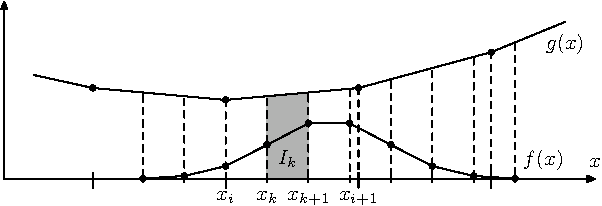
\includegraphics{integration.pdf}
  \caption{Schematic of antenna and backend calculations. The dashed 
    lines show the end points of each integral interval. The
    shaded area corresponds to the interval considered in
    Equation \ref{eq:sensor:weight:part integr}.}
  \label{fig:sensor:weight}
\end{center}
\end{figure}

\subsection{Summation}
\label{sec:sensor:sum}
The summation takes place when the mixer downconverts the sideband
signals into the intermediate frequency, $\nu_\mathrm{IF}$. This is
done by mixing the measurement signal with the local oscillator signal
(LO).  For a frequency $\nu$, the intermediate frequency is given by
\begin{equation}
  \label{eq:sensor:sum:v_if} 
  \nu_\mathrm{IF} = \vert \nu - \nu_\mathrm{LO} \vert,
\end{equation}
where $\nu_\mathrm{LO}$ is the frequency of the LO. This procedure has
the consequence that frequencies with the same distance to
$\nu_\mathrm{LO}$ are translated to the same $\nu_\mathrm{IF}$. Thus,
the `image' frequency, $\nu'$, corresponding to $\nu$ is
\begin{equation}
  \label{eq:sensor:sum:RF2IF}
  \nu' = 2\nu_\mathrm{LO} - \nu.
\end{equation}
The signal from $\nu$ and $\nu'$ is normally not weighted equally.
This can be an effect of a frequency dependent response of elements from
the antenna to the mixer, or caused by a sideband filter, with the
purpose of minimising the contribution from one of the bands. These
terms are here lumped together into one term, the sideband response
$w_\mathrm{sb}$. The apparent intensity after the mixer,
$I_\mathrm{IF}$, can then be expressed as
\begin{equation}
  \label{eq:sensor:sum:I_IF} 
  I_\mathrm{IF}(\nu_\mathrm{IF}) = \frac{w_\mathrm{sb}(\nu)I(\nu) + 
    w_\mathrm{sb}(\nu')I(\nu')}{w_\mathrm{sb}(\nu) + w_\mathrm{sb}(\nu')}.
\end{equation} 

To model the sideband folding, a vector $\mathbf{h}$ representing
the summation of the sideband filtered radio frequency (RF) signals
into an intermediate frequency (IF) signal is to be determined. The
translation of frequencies is given by Equation~\ref{eq:sensor:sum:RF2IF}. To
preserve all spectral information it is needed that the IF grid
includes all unique transformations from RF to IF. That is, the IF
grid shall be constructed by the projection of the RF grid from both
sidebands (with duplicates of IF values removed). This implies that
each IF grid point corresponds directly to a RF of one of the
sidebands, but will normally fall between RF grid points in the
other band, as illustrated in Figure~\ref{fig:sensor:folding}, 
if not the RF grid is perfectly symmetric around the LO frequency.

\begin{figure}
\begin{center}
  \includegraphics*{folding.pdf}
  \caption{Visualisation of how the RF sidebands are folded around $\nu_\mathrm{LO}$ down to the IF. 
           The sideband filter function, $w_\mathrm{sb}$, shows how the sidebands are weighted.}
  \label{fig:sensor:folding}
\end{center}
\end{figure}

 
Using a vector representation $\mathbf{v}$ of the RF grid and let
$\mathbf{v}_i$ and $\mathbf{v}_{i+1}$ encompass the frequency $\nu$
and $\mathbf{v}_j$ and $\mathbf{v}_{j+1}$ encompasses $\nu'$, then the
same notation as in Equation \ref{eq:sensor:sum:I_IF} can be used to
write the elements of the response vector $\mathbf{h}$ as
\begin{eqnarray}
\mathbf{h}_i & = & \frac{\mathbf{v}_{i+1}-\nu}
     {\mathbf{v}_{i+1}-\mathbf{v}_i} 
     \frac{w_\mathrm{sb}(\nu)}{w_\mathrm{sb}(\nu)+w_\mathrm{sb}(\nu')}, \\
  \mathbf{h}_{i+1} & = & \frac{\nu-\mathbf{v}_i}
     {\mathbf{v}_{i+1}-\mathbf{v}_i} 
     \frac{w_\mathrm{sb}(\nu)}{w_\mathrm{sb}(\nu)+w_\mathrm{sb}(\nu')}, \\
  \mathbf{h}_j & = & \frac{\mathbf{v}_{j+1}-\nu'}
     {\mathbf{v}_{j+1}-\mathbf{v}_j} 
     \frac{w_\mathrm{sb}(\nu')}{w_\mathrm{sb}(\nu)+w_\mathrm{sb}(\nu')}, \\
  \mathbf{h}_{j+1} & = & \frac{\nu'-\mathbf{v}_j}
     {\mathbf{v}_{j+1}-\mathbf{v}_j} 
     \frac{w_\mathrm{sb}(\nu')}{w_\mathrm{sb}(\nu)+w_\mathrm{sb}(\nu')},
\end{eqnarray} 
where all other elements of $\mathbf{h}$ are zero. Either $\mathbf{h}_{i+1}$ or
$\mathbf{h}_{j+1}$ is unnecessary to compute, depending on if the
IF corresponds directly to $\mathbf{h}_{i}$ or $\mathbf{h}_{j}$.
The complete response matrix is computed by iterating over all IF.

The normal situation should be that the sideband folding and
filtering are kept constant, and it is not needed to repeat the
calculations even if the instrument is scanning. The weights of
$\mathbf{h}$ from one viewing direction can for such cases be
applied throughout the scan.

%----------------------------------
\section{Instrument characteristics}
\label{sec:sensor:instchar}
To be able of computing the response from a certain sensor part, we
need the instrument characteristics. This information thus have to be
stored in such a way that we can incorporate it in our forward
model. ARTS uses XML-files to store and retrieve variables from files
and this offer a easy way to include characteristics that has been
prepared outside ARTS.  There also exist methods for computing simple
gaussian characteristics. See Section~\ref{sec:sensor:instchar:gauss}
below for more details.

To describe sensor characteristics in ARTS matrices are often used
with the first column containing relative grid positions for the
values in the following columns. These grid positions can for example
be frequencies relative to a channel frequency or angles relative to a
antenna line-of-sight. These matrices can then be grouped together in
arrays, or even array of arrays, to enable the characteristics to vary
with other parameters such as polarisation, and use of different
antennas. Common to all these variables are that the user has the
choice that for each parameter either provide one set of
characteristics that will be used for all cases or to provide a set of
characteristics for each state of the parameter. As an example,
consider the array of matrices used for the backend response
characteristics. On the matrix level, the first column holds the
relative frequency grid and the following hold the response values. If
we want the same response for all channel frequencies only one column
of response values is needed, on the other hand if we want the backend
response to vary with the channel frequencies a column must be given
for each frequency in $\nu_b$. Further on the array level, if the
array only has one matrix that response will be used for all
polarisations otherwise the array needs as many matrices as
polarisations simulated. Note that polarisations is not the same as
Stokes dimension, see Section~\ref{sec:sensor:pol} for more
information on polarisation.  How the sensor characteristics are
implemented for each sensor part are described in the sections
concerning the different sensor parts and in the online help.

\subsection{Gaussian response}
\label{sec:sensor:instchar:gauss}
There exist a simple method for creating a gaussian instrument
characteristic. Given the FWHM and the total width and maximum spacing
of the grid \artsstyle{GaussianResponse} creates a matrix where the
first column holds the relative grid and the second holds the
weights. This method has a limited use, but can prove useful for
setting up the characteristics for simple sensor configurations.

\subsection{Normalisation}
In most cases the sensor characteristics should be normalised as in
Equation~\ref{eq:sensor:weight:antenna},
\ref{eq:sensor:weight:spectrometer} and \ref{eq:sensor:sum:I_IF}, but
for the possibility to study the sensor response, the normalisation is
controlled by the WSV \artsstyle{sensor\_norm}. For normalised sensor
responses this variable should be set to one, and for non-normalised
sensor responses it should be zero.

%--------------------------------------
\section{Sensor response initialisation}
Even if the monochromatic pencil beam spectrum is studied without any
sensor influence, the sensor variables, especially \SnsMtr\ has to be
set. The reason is that the radiative transfer calculations allways
applies a \SnsMtr\ to the spectrum or spectra. On the other hand if a
response from a sensor system should be applied to the spectral values
the sensor variables has to be initialised properly. For these tasks
there exist two WSMs, \artsstyle{sensorOff} and
\artsstyle{sensor\_responseInit}. At least one of these has to be
included in the control file.

\subsection{No sensor}
If the calculated monochromatic pencil beams is to be studied as is,
i.e.~there is no sensor system present in the simulation, only one WSM
is needed \artsstyle{sensor\_off}. It sets all the necessary sensor
variables so that the monochromatic pencil beams are unchanged. This
means for instance setting \SnsMtr\ to be an identity matrix. This
method also affects several other workspace variables, to get a
complete list use the online help for \artsstyle{sensor\_off}. The
syntax to disable the sensor in the simulation is simply;
\begin{code}
sensorOff{}
\end{code}

\subsection{Initialisation}
When there is a sensor system present in the simulation the sensor
response variables has to be set up in a correct way. The WSM
\artsstyle{sensor\_responseInit} takes care of this. It sets the
\SnsMtr\ to be an identity matrix with correct size so that it is
applicable to the monochromatic pencil beam column vector. It also
initialises WSV that are use to remember the current settings of the
spectra, these are updated by all succeeding sensor response WSMs, and
therefor gives the accurate output grids and values for the frequency
and zenith- and azimuth angle grids and number of polarisations for
the final spectra. These variables are

\begin{tabular}{l l}
\artsstyle{sensor\_response\_f} & the frequency grid \\
\artsstyle{sensor\_response\_za} & the zenith angle grid \\
\artsstyle{sensor\_response\_aa} & the azimuthal angle grid \\
\artsstyle{sensor\_response\_pol} & the number of polarisations.
\end{tabular}

For the initial sensor response the output grids are the frequency
grid of the monochromatic pencil beam calculations, the zenith- and
azimuthal angle grid for each measurement block and the number of
polarisation equal the Stokes dimension. Since these WSV are used for
the initialisation they have to be set prior to calling
\artsstyle{sensor\_responseInit} together with
\artsstyle{sensor\_norm}, the position and line-of-sight of the sensor
and the atmosphere dimension.


%------------------------
\section{Antenna response}
\label{sec:sensor:antenna}
The influence of the antenna can as described above in
Equation~\ref{eq:sensor:weight:antenna} be expressed as a weighting
between the antenna response, $w_\mathrm{a}$, as a function of viewing
direction and the monochromatic pencil beam spectra.  In ARTS the
pencil beams are calculated for each measurement block at the angles
given by zenith- and azimuthal angle grids added to the current
line-of-sight as described in \ref{sec:fm_defs:sensorchar}. Which
viewing directions that are taken into account in the weighting is
determined by the antenna line-of-sight and the antenna pattern. ARTS
is prepared to handle a full 3D environment with a 2D antenna, but so
far only methods for 1D antennas have been developped.

\subsection{Antenna diagram}
\label{sec:sensor:antenna:diagram}
The antenna pattern $w_\mathrm{a}$ in ARTS is represented by a
structure \artsstyle{antenna\_diagram} that consists of an array of
arrays of matrices. The reason to use such a complicated structure is
to enable as much variability as possible when describing the antenna
pattern. With this structure it is possible to define the antenna
response for different viewing angles, polarisations and frequencies.
Since there only exists a method for 1D antennas, $w_\mathrm{a}$ is so
far only defined for 1D antenna patterns. The structure consists of
matrices that describe the weights for different angles. The first
column in matrices describes the relative angular grid and the
following columns the weights for different frequencies, see
Figure~\ref{fig:sensor:ant_diag}. Combining the antenna patterns
relative angular grid with the antenna line-of-sight relative angle
gives the measurement block angular grid seen by the antenna. Each
polarisation is then represented by a separate matrix and each viewing
angle by an array of matrices. By using arrays of matrices instead of
tensors it is also possible to use different settings for the
different polarisations/viewing directions. For each of these sets it
is possible to define only one column, matrix or array of matrices, or
a full set of columns, matrices or arrays of matrices. E.g.~for the
most simple case where the antenna has the same pattern for all
directions and frequencies $w_\mathrm{a}$ consists of a single array
of matrix with a single two column matrix.
\begin{figure}
\label{fig:sensor:ant_diag}
\begin{center}
  \includegraphics*{ant_diag}
  \caption{Visualisation of the antenna pattern WSV \artsstyle{antenna\_diagram} for   
  two viewing directions $\varphi_1$ and $\varphi_2$, $\Delta\varphi$ is the relative   
  angular grid, $f_i$ the $i$:th frequency and $p_j$ the $j$:th polarisation.}
\end{center}
\end{figure}

\subsection{Antenna line-of-sight}
As described in \ref{sec:sensor:antenna:diagram} the antenna pattern
includes a dimension for different viewing directions. This is useful
when simulating multiple antennas or a multiple beam antenna. The
viewing directions are described in ARTS by
\artsstyle{antenna\_los}. This is a one- or two column matrix
describing the relative offset of the antennas with respect to the
sensor line-of-sight. The columns follow the general idea for antenna
dimensionality, with first column denoting zenith offsets and the
second being used for 2D antennas and denoting azimuthal offsets. The
rows on the other hand describes the number of antennas or beams, and
in the common case of only one antenna present the matrix should
therefor contain a row of zero.  This variable is important when
dealing with rotating sensors as is described in
Section \ref{sec:sensor:pol:rotation}.

\subsection{1D antenna}
Here it will be assumed that the variation of \Mpi\ in one angular
dimension can be neglected, and that the weighting can be described by
an one dimensional integral:
\begin{eqnarray}
\label{eq:sensor:antenna:1D}
  \aMpi{\mathrm{a}} &=& \int_{-\pi}^\pi\!\!\!\!I(\theta+\theta_0) 
  w_\mathrm{a}^\theta(\theta)\;\mathrm{d}\theta,\\
  w_\mathrm{a}^\theta(\theta) &=& \int_0^{2\pi}\!\!\!\!
  w_\mathrm{a}(\theta,\phi)\cos(\theta)\,\mathrm{d}\phi,
\end{eqnarray}
where $\theta_0$ is the reference angle of the antenna, the weighting
is only performed over the zenith angles. The only variables needed
apart from the variables needed for the initialisation are the antenna
line-of-sight and the antenna pattern. A convenient way to set the
antenna dimensionality before the sensor initialisation is to use the
WSM \artsstyle{AntennaSet1D}.

The 1D antenna is included in the sensor by using the WSM
\artsstyle{sensor\_responseAntenna1D} and it updates both \SnsMtr\ and
the zenith angular grid of the final spectra.


%-----------------------------
\section{Polarisation and rotation}
\label{sec:sensor:pol}
Taking polarisation into account, and assuming no losses, the measured
intensity for a certain direction and frequency , $I_p$, is
\begin{equation}
\label{eq:sensor:pol:response}
  I_\mathrm{p} = \frac{1}{2} \mathbf{p} \mathbf{s}
\end{equation}
where $\mathbf{s}$ is the Stokes components of the incoming radiation
and $\mathbf{p}$ is a row vector of the same length as $\mathbf{s}$
describing the sensor polarisation response. For a rotating sensor a
transformation matrix \MtrStl{L}$(\chi)$, see
Section \ref{sec:sensor:pol:rotation}, is applied to obtain consistent
definition between the polarisation directions for atmospheric
radiation and sensor response, Equation \ref{eq:sensor:pol:response}
then becomes
\begin{equation}
\label{eq:sensor:pol:rotpolrespons}
  I = \frac{1}{2} \mathbf{p} \mathbf{L}(\chi) \mathbf{s}.
\end{equation}
For an instrument measuring a single polarisation, the first element
of $\mathbf{p}$ shall be one and the three last elements shall fulfil
$\sum_{i=2}^4 p_i^2 = 1$, where $p_i$ is the $i$:th element of
$\mathbf{p}$. For example, if vertical polarisation is measured, then
$\mathbf{p}=[1\ 1\ 0\ 0]$ and for linear $\pm45^\circ$ polarisation
$\mathbf{p}=[1\ 0\ \mp\!\!1\ 0]$.

Several sensor parts can have a polarisation varying response, but
there is normally a single part that dominates the polarisation
response. The normal case for the instrument type considered here is
that the mixer is only sensitive to a single polarisation, and the
natural time to apply Equation \ref{eq:sensor:pol:response} or
\ref{eq:sensor:pol:rotpolrespons} is then after the antenna, but
before the sideband folding and the backend.

\subsection{Polarisation response}
\label{sec:sensor:pol:polarisation}
To study different polarisations in ARTS, these has to be defined by
the polarisation matrix \MtrStl{P}. This is a matrix where each row is
a row vector $\mathbf{p}$ corresponding to the polarisation to study
and the columns matches the Stokes components of the simulation. The
number of columns must therefor equal the Stokes dimension of the
simulation, see Section \ref{sec:polarization} for more information
and especially Section \ref{sec:polarization:measuring} for examples
of some standard polarisations. An example matrix for studying
horisontally and right-handed circular polarisation would look like
\begin{displaymath}
  \MtrStl{P} = \left[ \begin{array}{c c c c}
  1 & -1 & 0 & 0 \\ 1 & 0 & 0 & 1 \\ 
  \end{array} \right].
\end{displaymath}
When initialised \MtrStl{P} is set to be the identity matrix, so to
study all Stokes components nothing more has to be done.  The
\artsstyle{sensor\_pol} matrix is most easily read from XML-file, and
the calculation of the sensor response of polarisation is done by
calling \artsstyle{sensor\_responsePolarisation}. After this method
the number of polarisations are equal to the rows of \MtrStl{P}. When
applying a polarisation matrix to the monochromatic pencil beam
spectra the intensities are no longer ordered by Stokes dimension,
instead they get ordered by the polarisations given in \MtrStl{P}.

\subsection{Rotating sensor}
\label{sec:sensor:pol:rotation}
A rotating sensor configuration can be modelled by rotating the sensor
frame between each measurement block by an angle $\chi$. The
transformation matrix for an angle $\chi$ is given by \cite{liou:02},
\begin{equation}
  \label{eq:sensor:polrot}
  \mathbf{L}(\chi) = \left[ \begin{array}{cccc}
    1 & 0           & 0          & 0 \\
    0 & \cos 2\chi  & \sin 2\chi & 0 \\
    0 & -\sin 2\chi & \cos 2\chi & 0 \\
    0 & 0           & 0          & 1 \\
  \end{array} \right].
\end{equation}

In ARTS the rotation angles $\chi$ is stored in the vector
\artsstyle{sensor\_rot}, and is used to assign a rotation angle for
each antenna line-of-sight. If the rotation is constant the
\artsstyle{sensor\_rot} vector can contain a single element describing
that rotation angle. From Equation \ref{eq:sensor:pol:rotpolrespons}
it can be seen that the rotation should be applied to the incoming
intensities before the polarisation, therefor the call to
\artsstyle{sensor\_responseRotation} must precede the call to the
polarisation WSM in the control file. Since the rotation WSM does not
know anything about viewing directions it must also be placed after
the antenna function.


%------------------------------------------
\section{Mixer and sideband filter response}
As described in Section \ref{sec:sensor:sum} the mixer folds the two
RF sidebands together into the IF band. At the same time the sideband
ratio can be altered by the mixer itself and a sideband filter, these
two effects are grouped together to what we refer to as the sideband
filter. In ARTS there are methods both for a single mixer
configuration and for multiple mixer configurations. From
Equation \ref{eq:sensor:sum:I_IF} it can be seen that the summation is
by its definition normalised, so even if \artsstyle{sensor\_norm} is
set to one the rows of \aSnsMtr{\mathrm{mixer}} will be normalised.

\subsection{Single mixer and sideband filter}
For the single mixer configuration the needed variables are the LO
frequency, $\nu_\mathrm{LO}$, and the sideband filter function,
$w_\mathrm{sb}$. In ARTS the $\nu_\mathrm{LO}$ is stored in the vector
\artsstyle{lo} which in this case should have length one, and
$w_\mathrm{sb}$ is given as a matrix, the first column holding the RF
grid and the second column the weights. There are no special WSV
dedicated for the sideband filter, so it needs to be loaded into the
arbitrary matrix variable \artsstyle{matrix\_1} before being passed as
a generic input to the calculating routine. This could look like
\begin{code}
ReadXML( lo ) { "lo.xml" }
ReadXML( matrix_1 ) { "sbfilter.xml" }
sensor_responseMixer( matrix_1 ) {}
\end{code}
The method \artsstyle{sensor\_responseMixer} changes the sensor
response grid for frequencies to be in IF, this grid is also stored in
\artsstyle{f\_mixer}. Depending on the RF grid configuration, the
conservation of all spectral values in RF may increase the number of
grid points in IF.

\subsection{Multiple mixers with single backends}
For a sensor configuration with several channels which are related to
different mixers a special WSM have been designed
\artsstyle{sensor\_responseMultiMixerBackend}.  This method works a
bit different from the individual mixer and backend WSM. In this
method each channel is related to a polarisation state, a local
oscillator and a backend frequency channel. These three variables have
to be declared for each channel, even if they are equal for some of
the channels.
% For a sensor configuration studying more than one polarisation it is sometimes desirable to specify several different mixers. To make this efficient the backend response is also added directly to the mixer response, and this is handled by the method \artsstyle{sensor\_responseMultiMixerBackend}. 
The WSV that hold these variables are \artsstyle{sensor\_pol},
\artsstyle{lo} and \artsstyle{f\_backend}, and these should all have
the same number of rows/length.  For each channel the specified
polarisation state is constructed from the Stokes vector, and a
\aFrq{\mathrm{LO}} is specified folding the spectra as in
Equation \ref{eq:sensor:sum:I_IF}. The $w_\mathrm{sb}$ can be given
different weights for the different channels, these have to be given
for the same relative grid and should be stored as subsequent columns
in the generic input matrix.  This method also applies the backend
response to the spectra, this means a weighting over frequencies see
Equation \ref{eq:sensor:weight:spectrometer}, with the possibility of
using different backend responses for the different channels. Formally
we can write the resulting sensor response as the product of the mixer
and backend responses,
\begin{equation}
\aSnsMtr{\mathrm{out}} = \aSnsMtr{\mathrm{backend}} \aSnsMtr{\mathrm{mixer}}
\end{equation}
This implies that the backend channel characteristics, $w_\mathrm{b}$,
and the channel frequencies, \aFrq{\mathrm{ch}}, has to be stored in
their WSV prior to calling the WSM. This method operates in RF
therefore \aFrq{\mathrm{ch}} also has to be given in that domain, this
also set the new sensor response frequency grid to be in RF. An
important difference to the \artsstyle{sensor\_responseBackend} method
is that the backend response is given as a single matrix instead of an
array of matrices. For more information about the backend response see
Section \ref{sec:sensor:backend}.

\subsection{Conversion of IF to RF}
Since the mixer methods change the sensor response grid into IF, it
can sometimes be convenient to be able to convert them back into the
RF domain for a more understandable result. This is also a necessary
step to perform if the radiances are to be converted into brightness
temperatures. The conversion is done by the method
\artsstyle{ConvertIFToRF} that given the generic input for which
sideband to return, changes the sensor response frequency grid and if
necessary re-orders the spectral values. If the IF grid is unfolded to
double sidebands the number of grid points in RF will be twice as many
as in IF, thus increasing the size of the sensor response frequency
vector and the measurement vector. This method only works for single
mixer configurations where there is only one $\nu_\mathrm{LO}$ given.


%------------------------
\section{Backend response}
\label{sec:sensor:backend}
The last sensor part in the instrument is generally called the
backend, sometimes the mixer is also included in this concept but here
we only consider the part that transform monochromatic radiances into
channel frequency radiances. In the case of a radiometer, this can be
a spectrometer. Like the antenna weights the monochromatic pencil
beams over angles, the backend spectrometer performs a similar
weighting over frequencies as described by
Equation \ref{eq:sensor:weight:spectrometer}. The spectra goes from
being monochromatic to include intensities from the neighbouring
frequencies.  In ARTS the weighting is controlled by two variables;
the channel centre frequencies \aFrq{\mathrm{ch}} and the spectrometer
channel response $w_\mathrm{ch}$. The channel centre frequencies are
the frequencies for which the spectrometer outputs the measured
radiances, for this purpose the WSV \artsstyle{f\_backend} is a vector
that has to be provided by the user.  The spectrometer channel
response describes how the monochromatic radiances are weighted around
the centre frequencies, in analogy with the antenna line-of-sight and
antenna pattern. The channel response is stored as an array of
matrices, this way the weights are allowed to vary with frequency and
polarisation. The matrices consists of a relative frequency grid and
subsequent weights. Each matrix corresponds to the polarisations given
in \MtrStl{P}. The $w_\mathrm{ch}$ array of matrices can be passed to
\artsstyle{sensor\_responseBackend} by the generic input
\artsstyle{arrayofmatrix\_1}. This WSV can be set up by reading
XML-files or by calling the function \artsstyle{ArrayOfMatrixSet}, see
the online help for instructions.  After applying the sensor response
for the backend spectrometer the sensor response frequency grid is
updated to be equal the \aFrq{\mathrm{ch}} grid.
% \begin{code}
% ReadXML( matrix_1 ) {
%   "../xml/ac_channel.xml"
% }
% 
% ArrayOfMatrixSet( arrayofmatrix_1, matrix_1 ) {
%   element = 0
% }
% 
% sensor_responseBackend( arrayofmatrix_1 ) {}
% \end{code}


%------------------------
\section{Control file example}

% \hrule


%-------------------------
% \section{Workspace methods}
% \label{sec:sensor:WSM}

%------------------------------------------------------
% \section{Controlfile implementation(flow, step-by-step)}



%\section{Implementation strategy}
% \label{sec:sensor:strategy}

%\subsection{The sensor transfer matrix}
% \label{sec:sensor:strategy:h}
 
% The modeling of a sensor part is either a summation of different
% frequency components (mixer), or a weighting of the spectra as a
% function of frequency (spectrometer) or viewing direction (antenna)
% with the instrument response of concern. In all cases it is
% possible to describe the sensor influence by an analytical
% expression. See for example \citet{eriksson:97a} for more details.
% These analytical expressions can be implemented and solved for each
% run of the sensor model, but this would be relatively computationally
% demanding for cases when the settings are kept constant, as the
% calculations are duplicated in an unnecessary manner, and we want to
% find a better implementation strategy.
 
% Summation and weighting of the spectral components are both linear
% operations, and thus it is possible to model the effect of the
% different sensor parts as subsequent matrix multiplications of the
% monochromatic pencil beam spectrum, as suggested in \citet{eriksson:00a}:
% \begin{eqnarray}
%   \MsrVct = \Hm_n\dots\Hm_2\Hm_1\iv + \merr
% \end{eqnarray}
% where $n$ is the number of sensor parts to consider, and this results
% in that the sensor model can be expressed as a single matrix
% multiplication (Eq. \ref{eq:formalism:H})
% \begin{eqnarray}
%   \MsrVct = \Hm\iv + \merr                     \nonumber
% \end{eqnarray}
% Applying Equation \ref{eq:formalism:H} for the sensor model will
% clearly give very rapid calculations, and we must find ways to
% calculate $\Hm$.


%\subsection{Normalization of \Hm}
% \label{sec:sensor:strategy:norm}
 
% It is important that the transfer matrix for
% each sensor part is normalized in such way that a unit response is
% obtained. A unit response signifies here that a constant intensity
% (as a function of frequency or zenith angle) is preserved, that is
% \begin{equation}
%   \mat{u}_2 = \Hm\mat{u}_1
% \end{equation}
% where $\mat{u}_1$ and $\mat{u}_2$ are vectors of appropriate length
% where each element is $1$. This criterion equals that the sum of 
% the elements of each row of \Hm\ is 1.


%\section{Integration as vector multiplication} 
% \label{sec:sensor:integr}
  
% The effect of both the antenna and the spectrometer can be expressed
% as an integral \citep[e.g.][Eq. 86 and 94]{eriksson:97a}, and the
% question is how to transform these integrals into matrix operations.
  
% The problem at hand is that the antenna and spectrometer responses
% and the zenith angle and frequency grids are known, while the spectral
% values are unknown. This problem corresponds to determine a (row)
% vector $\mat{h}$ that multiplied with an unknown (column) vector,
% $\mat{g}$, approximates the integral of the product between the
% functions $g$ and $f$:
% \begin{equation} 
%   \mat{hg} = \int{f(x)g(x) \dd x}
%   \label{eq:sensor:integral_problem}
% \end{equation}
% where $\mat{g}$ contains values of $g$ at some discrete points. The
% functions $f$ is here the response for some sensor part, and $g$
% holds the spectral values. The shape of $f$ and $g$ between the grid
% points must be known to solve this problem.


%\subsection{Piecewise linear functions} 
% \label{sec:sensor:integr:lins}
 
% In this section the problem of
% Equation \ref{eq:sensor:integral_problem} is solved analytically when
% both functions are piecewise linear. The practical solution used
% Qpack is discussed in next section.
  
% Following Figure \ref{fig:sensor:vecintegr}, the function $g$ can between
% the points $x_1$ and $x_4$ be expressed as a sum of the two unknown
% values $g_1$ and $g_2$:
% \begin{equation}
%   g(x) = g_1 + (g_2-g_1)\frac{x-x_1}{x_4-x_1} =
%           g_1 \frac{x_4-x}{x_4-x_1} + g_2\frac{x-x_1}{x_4-x_1}
% \end{equation}
% which can be rewritten as
% \begin{equation}
%   g(x) = g_1(a+bx)+g_2(c-bx), \qquad x_1 \leq x \leq x_4
%   \label{eq:sensor:glin}
% \end{equation}
% where
% \begin{eqnarray}
%    a=\frac{x_4}{x_4-x_1}, \qquad b=\frac{-1}{x_4-x_1}, \qquad 
%    c=\frac{-x_1}{x_4-x_1}   \nonumber
% \end{eqnarray} 
% A shorter expression can be obtained for the function $f$ as the
% values $f_1$ and $f_2$ are known:
% \begin{equation}
%   f(x) = (d+ex), \qquad x_2 \leq x \leq x_3
% \end{equation}
% where 
% \begin{eqnarray}
%    d=f_1-x_2\frac{f_2-f1}{x_3-x_2} \qquad e=\frac{f_2-f_1}{x_3-x_2} \nonumber
% \end{eqnarray}
% \begin{figure}[tb]
%    \begin{center}
%      \includegraphics*{vecintegr}
%      \caption{The quantities used in Section \ref{sec:sensor:integr}.}  
%      \label{fig:sensor:vecintegr} 
%    \end{center} 
% \end{figure}
% The integral in Equation \ref{eq:sensor:integral_problem} can now for
% ranges between $x_2$ and $x_3$ be calculated analytically in a
% straightforward manner:
% \begin{eqnarray}
%    \int_{x_a}^{x_b}{f(x)g(x) \dd x} =
%    \int_{x_a}^{x_b}{\big(d+ex\big)\big(g_1(a+bx)+g_2(c-bx)\big) \dd x}  
%    =\dots= \nonumber\\
%    \bigg[ g_1x\Big(ad+\frac{x}{2}(bd+ae)+\frac{x^2}{3}be\Big) + 
%           g_2x\Big(cd+\frac{x}{2}(ce-bd)-\frac{x^2}{3}be \Big)
%           \bigg]_{x_a}^{x_b}
%    \label{eq:sensor:integr_weights}
% \end{eqnarray}
% For the practical calculations, the integral is solved from one grid
% point to next, of either $\mat{f}$ or $\mat{g}$. The functions are 
% assumed to be zero outside their defined ranges (for example, $f=0$ 
% for $x<x_2$).
% For the case
% shown in Figure \ref{fig:sensor:vecintegr}, the integration order would be
% $(x_a,x_b)=(x_2,x_3)$, $(x_a,x_b)=(x_3,x_4)$, $(x_a,x_b)=(x_4,x_5)$
% \ldots\
  
% Using Equation \ref{eq:sensor:integr_weights}, we can now determine how to
% calculate $\mat{h}$. For each integration step, $\mat{h}_i$ and
% $\mat{h_{i+1}}$ are increased as
% \begin{eqnarray}
%    \mat{h}_i \!\! &=& \!\! \mat{h}_i +    
%              x_b\Big(ad+\frac{x_b}{2}(bd+ae)+\frac{x_b^2}{3}be\Big) - 
%              x_a\Big(ad+\frac{x_a}{2}(bd+ae)+\frac{x_a^2}{3}be\Big) 
%    \nonumber \\
%    \mat{h}_{i+1} \!\! &=& \!\! \mat{h}_{i+1} +
%              x_b\Big(cd+\frac{x_b}{2}(ce-bd)-\frac{x_b^2}{3}be\Big) - 
%              x_a\Big(cd+\frac{x_a}{2}(ce-bd)-\frac{x_a^2}{3}be\Big) 
%    \nonumber
% \end{eqnarray}
% where $i$ is the index for which $\mat{x}^i \leq x_a$ and $x_b \leq
% \mat{x}^{i+1}$. The vector $\mat{h}$ is initialized with
% zeros before the calculation starts.


%\subsection{Practical solution} 
% \label{sec:sensor:integr:practical}
 
% The functions $f$ and $g$ can in Qpack be treated to be piecewice
% linear or cubic functions. The polynomial order of the two functions
% is set individually. When a function is assumed to be piecewise
% cubic, two points on each side of the range of interest (that is, in
% total 4 points) are used to determine the polynomial. For the end
% ranges, a quadratic polynomial is used as there exists only a single
% point on one of the sides. 
 
% Accordingly, Equation \ref{eq:sensor:integral_problem} must be
% handled in Qpack for combinations of piecewise linear, quadratic and
% cubic functions. Instead of repeating the calculations in Section
% \ref{sec:sensor:integr:lins} for all possible polynomial
% combinations, a more general solution was implemented. The polynomial
% coefficents for $f$ are simply obtained by doing a polynomial fit to
% the considered points (by the Matlab function \verb|polyfit|). The
% polynomial basis for $g$ ($a$, $b$ and $c$ in Equation
% \ref{eq:sensor:glin}) is obtained by Lagrange's formula (Equation
% \ref{eq:wfuns:lagrange}), which expresses the polynomial that passes
% a fixed set of points. The Lagrange's formula can be written as:
% \begin{eqnarray}
%  g(x) &=& (a_{11}+a_{12}x+\dots+a_{1N}x^N)*g_1 + \nonumber \\
%       & & (a_{21}+a_{22}x+\dots+a_{2N}x^N)*g_2 + \nonumber \\
%       & & \dots \nonumber \\
%       & & (a_{N1}+a_{N2}x+\dots+a_{NN}x^N)*g_N 
%  \label{eq:sensor:pbasis}
% \end{eqnarray}
% With the obtained coefficients for $f$ and $g$, Equation
% \ref{eq:sensor:integr_weights} can easily be solved analytically in a
% general manner. The polynomial pasis is determined by the AMI
% function \verb|pbasis|, the both set of coefficients are
% multiplicated in the function \verb|pbasis_x_pol| and the integral is
% solved by the function \verb|pbasis_integrate|.


%\section{Summation as vector multiplication}
% \label{sec:sensor:mixer}
  
% The influence of the mixer and sideband filter of the sensor
% correspond to a summation of pairs of frequency components. The two
% frequencies of the pair are related as
% \begin{equation}
%    \f' = 2\f_{LO}-\f
% \end{equation}
% where $\f_{LO}$ is the frequence of the local oscillator signal, and
% $\f'$ is denoted as the image frequency.

% \begin{figure}[tb]
%  \begin{center}
%    \includegraphics*[width=0.8\hsize]{sideband}
%    \caption{Schematic description of image frequency and sideband filtering.}
%   \label{fig:sensor:sideband} 
%  \end{center} 
% \end{figure}
 
% The intensity correspondence after the mixer and the sideband filter
% can be written as
% \begin{equation}
%   I_{IF}(\f) = \frac{f_s(\f)I(\f)+f_s(\f')I(\f')}{f_s(\f)+f_s(\f')}
%  \label{eq:sensor:sband}
% \end{equation}
% where $I(\f)$ is the intensity for frequency $\f$ and $f_s$ the response
% of the sideband filter as a function of frequency.

% The frequency grid after the mixer consists of the frequencies inside
% the primary band of the grid before the mixer. To include frequencies
% from the image band (mirrored to the primary band) would need an 
% interpolation in the primary band that could cause unexpected effects.  


%\subsection{Piecewise linear functions} 
% \label{sec:sensor:mixer:lins}

% If the intensity is assumed to vary linearly between the points of the
% frequency grid, Equation \ref{eq:sensor:sband} can be written as
% \begin{eqnarray}
%   I_{IF}(\f^i) &=& \frac{1}{f_s(\f_i)+f_s(\f_i')} \bigg[ f_s(\f_i)I(\f_i)+ \nonumber \\ 
%      & & + \frac{f_s(\f_i')}{\f_{j+1}-\f_j} \Big( I(\f_j)(\f_{j+1}-\f_i')
%           + I(\f_{j+1})(\f_i'-\f_j) \Big)  \bigg]
%  \label{eq:sensor:mixer}
% \end{eqnarray}
% where $f_s$ for the different frequencies is obtained by linear
% interpolation, and $\f_j$ and $\f_{j+1}$ are the two
% points of the frequency grid surrounding the image frequency,
% $\f_i'$. The row of the $\Hm$ matrix corresponding to $\f^i$ is then
% \begin{eqnarray}
%    \label{eq:sensor:mixer:hi}
%    \mat{h}^i &=& \frac{f_s(\f_i)}{f_s(\f_i)+f_s(\f_i')}  \\
%    \mat{h}^j &=& \frac{f_s(\f_i')}{f_s(\f_i)+f_s(\f_i')}
%                  \frac{\f_{j+1}-\f_i'}{\f_{j+1}-\f_j}     \nonumber \\
%    \mat{h}^{j+1} &=& \frac{f_s(\f_i')}{f_s(\f_i)+f_s(\f_i')}
%                  \frac{\f_i'-\f_j}{\f_{j+1}-\f_j}     \nonumber
% \end{eqnarray}
% where $\mat{h}^i$ is the value of $\mat{h}$ for frequency $\f_i$ etc.
% Remaining values of $\Hm$ are zero.

% For the special case when the image frequency matches perfectly a frequency
% grid point, the equations above can be simplified to give
% \begin{eqnarray}
%    \mat{h}^i &=& \frac{f_s(\f_i)}{f_s(\f_i)+f_s(\f_i')}    \nonumber \\
%    \mat{h}^j &=& \frac{f_s(\f_i')}{f_s(\f_i)+f_s(\f_i')}    \nonumber
% \end{eqnarray}


%\subsection{Practical solution} 
% \label{sec:sensor:mixer:practical}
 
% The responses of the sideband filter is determined by linear or cubic
% interpolation, dependent on the selected order.
% As the frequency in the primary band always equals one of the points
% of the monochromatic frequency grid, Equation
% \ref{eq:sensor:mixer:hi} can be used throughout. The weights for the
% image band are found by evaluating the polynomial basis from Equation
% \ref{eq:sensor:pbasis} at $\f_i'$ and multiplicate with 
% $f_s(\f_i') / (f_s(\f_i)+f_s(\f_i'))$. These calculations are 
% performed in the AMI function \verb|h_matrix|.

 
%\section{Brightness temperature} 
% \label{sec:sensor:tb}

% Some kind of calibration process, either in absolute or relative units,
% is always needed. For mm and sub-mm receivers, the calibration normally
% presents the measured intensity in some temperature scale, and conversion
% to brightness and Rayleigh-Jeans temperatures is also treated in this section.


%\subsection{Conversion to Planck brightness temperature} 
% \label{sec:sensor:tb_planck}

% The brightness temperature is defined as the temperature a blackbody 
% shall have to give the same intensity magnitude as observed. The 
% brightness temperature is thus calculated as
% \begin{equation}
%   T_b = \frac{h\f}{k_B} \frac{1}{\ln{ \left( \frac{2h\f^3}{c^2\mpbi}+1 \right)}}
%   \label{eq:sensor:cal:tb}
% \end{equation}
% where \mpbi\ is the radiative intensity.
 
% It should be noted that the conversion from intensity to brightness
% temperature is non-linear. This non-linearity has (at least) two important
% consequences:
% \begin{itemize}
%  \item The conversion from intensity to brightness temperature cannot be
%        included in \Hm.
%  \item \bf{Brightness temperature cannot be used for retrievals.}
% \end{itemize}
% Accordingly, the main reason to convert a spectrum to brightness
% temperatures is to display the spectrum in an unit that gives a more
% intuitive understanding of the emission magnitude.


%\subsection{Conversion to Rayleigh-Jean temperature} 
% \label{sec:sensor:tb:rj}

% For lower frequencies where $h\f \ll k_BT$ the Planck function can
% be approximated by the Rayleigh-Jean (RJ) formula:
% \begin{equation}
%   B \approx \frac{2\f^2k_BT}{c^2}
% \end{equation}
% This relationship holds rather well in the microwave region. For example,
% for $T=50$~K, $h\f = k_BT$ at 1.04~THz. The RJ approximation of the Planck
% function gives a natural definition on a ``brightness temperature'' with
% that has a linear relationship to the intensity:
% \begin{equation}
%   T_{rj} = \frac{c^2}{2\f^2k_B} \mpbi
%   \label{eq:sensor:cal:rj}
% \end{equation}
% This intensity unit is often referred to as the brightness temperature but
% to avoid confusion it is here denoted as the RJ temperature.
 
% As the intensity from intensity to RJ temperature is linear, this
% conversion can be included in \Hm\ and weighting functions can be
% converted using \ref{eq:sensor:cal:rj}, that is, retrievals are
% possible using RJ temperatures.
% On the other hand, the RJ temperature shall not be mistaken for the
% ``physical'' brightness temperature $(T_b)$ as the deviation between
% $T_b$ and $T_{rj}$ is not negligible \citep{eriksson:97a}.


%\section{Control file examples}
% \label{sec:sensor:cfe}

% The following sequence of ARTS functions can be used to store the
% spectra in both brightness temperature units:

% \begin{code}
%VectorCopy( y0, y ) {
%}
%yTRJ{
%}
%VectorWriteAscii( y ) {
%   "ytb_rj.aa"
%}
%VectorCopy( y, y0 ) {
%}
%yTB{
%}
%VectorWriteAscii( y ) {
%   "ytb_planck.aa"
%}
% \end{code}
% \noindent
% A weighting function matrix is converted to Rayleigh-Jean temperature
% as:

% \begin{code}
%MatrixTRJ( kx, kx ) {
%}
% \end{code}
 


%%% Local Variables: 
%%% mode: latex 
%%% TeX-master: "uguide" 
%%% End:

